\documentclass[11pt, a4paper]{report}

\usepackage{fontspec}
\setmainfont[Script=Greek]{GFS Artemisia}
\setmonofont{FreeMono}

\usepackage{polyglossia}
\setdefaultlanguage{greek}
\setotherlanguages{english}

\usepackage{geometry}
\geometry{margin=3cm}

\usepackage{minted2}
\usepackage{graphicx}

\begin{document}

% header section
\author{Πλαστήρας Πέτρος}
\title{Εργασία \#2 - Μέρος B}
\date{\today}
\maketitle

% TODO: mention fastest and slowest path times not just the tables
\section{Άσκηση 1}
Σχεδιάστε ένα συνδυαστικό λογικό κύκλωμα σε VHDL το οποίο υλοποιεί τις ακόλουθες λογικές και αριθμητικές πράξεις (ALU) ανάλογα με τις τιμές των σημάτων $S_1, S_0, C_{in}$.

\begin{center}
	\begin{tabular}{|c|c|c|c|}
		\hline
		$S_1$ & $S_0$ & $C_{in}$ & Πράξη                           \\
		\hline
		0     & 0     & x        & $Y = A - B + C_{in}$            \\
		0     & 1     & x        & $Y = Shift Right Arithmetic(A)$ \\
		1     & 0     & 0        & $Y = Shift Logical Right(B)$    \\
		1     & 0     & 1        & $Y = Shift Logical Left(A)$     \\
		1     & 1     & x        & $Y = \overline{A \cdot B}$      \\
		\hline
	\end{tabular}
\end{center}

Σας δίνεται ο ορισμός της οντότητας:
\inputminted[firstline=5, lastline=14]{vhdl}{./code/part-2/alu-1/alu.vhdl}

Για την υλοποίηση της αρχιτεκτονικής της οντότητας, αφού το κύκλωμα είναι συνδυαστικό αρκεί να χρησιμοποιήσουμε μια  \\
αρχιτεκτονική μορφής Dataflow. Συγκεκριμένα, θα συνδυάσουμε τα σήματα $S_0$ και $S_1$ σε ένα σήμα \mintinline{vhdl}{std_logic_vector} των 2 bit, το οποίο ονομάζουμε $S$.
Στην συνέχεια με την χρήση μιας δομής \mintinline{vhdl}{with S select} θα μπορούμε να επιλέξουμε το αποτέλεσμα του κυκλώματός μας για τις διάφορες τιμές του $S$.

Τώρα για τον υπολογισμό των αποτελεσμάτων, θα χρησιμοποιοίσουμε τα παρακάτω:
\begin{enumerate}
	\item Αρχικά για την περίπτωση που $S = 00$, θα χρησιμοποιήσουμε τον τύπο \mintinline{vhdl}{signed} από το πακέτα \mintinline{vhdl}{numeric_std}.
	      Για να γίνει αυτό πρέπει να μετατρέψουμε το $A$, το $B$ και το $C_{in}$ σε \mintinline{vhdl}{signed}.
	      Το $C$ χρειάζεται αρχικά να μετατρεπεί από \mintinline{vhdl}{std_logic} σε \mintinline{vhdl}{std_logic_vector} των 8 bit.
	      Ύστερα μπορούμε απλά να αφαιρέσουμε το $A$ και το $B$ να προσθέσουμε το $C$ και να μετατρέψουμε το αποτέλεσμα πίσω σε \mintinline{vhdl}{std_logic_vector}.
	\item Στην περίπτωση που $S = 01$ θα μετατρέψουμε το $A$ σε \mintinline{vhdl}{signed} και στην συνέχεια θα χρησιμοποιήσουμε την συνάρτηση
	      \mintinline{vhdl}{shift_right} η οποία αν η είσοδός της είναι προσημασμένος, παραγματοποιεί αριθμητική ολίσθηση.
	\item Αν το $S = 10$ θα χρησιμοποιήσουμε ένα νέο εσωτερικό σήμα, το οποίο υλοποιεί την λογική της ολίσθησης ανάλογα με την τιμή του $C_{in}$.
	      Αν είναι 0, κάνει δεξιά ολίσθηση το σήμα $B$ ενώ αν είναι ένα κάνει αριστερή ολίσθηση το σήμα $A$. Το παραπάνω υλοποιείται επίσης με την χρήση μιας δομής \mintinline{vhdl}{with Cin select}.
	\item Τέλος, αν $S = 11$ μπορούμε άμεσα με την χρήση του τελεστή \mintinline{vhdl}{nand} να υλοποιήσουμε την πράξη $\overline{A \cdot B}$.
\end{enumerate}

Σύμφωνα μα τα παραπάνω προκύπτει ο παρακάτω κώδικας για την οντότητα $ALU$:
\inputminted[breaklines, linenos]{vhdl}{./code/part-2/alu-1/alu.vhdl}

Για το αρχείο της προσομοίωσης απλά ελέγχουμε κάποιες ενδεικτικές περιπτώσεις, με θετικούς και αρνητικούς αριθμούς:
\inputminted[breaklines, linenos]{vhdl}{./code/part-2/alu-1/alu_tb.vhdl}

\newpage

Αφού έχουμε κάνει τα παραπάνω μπορούμε να κάνουμε RTL ανάλυση της οντότητάς μας. Το αποτέλεσμα φαίνεται παρακάτω:
\begin{center}
	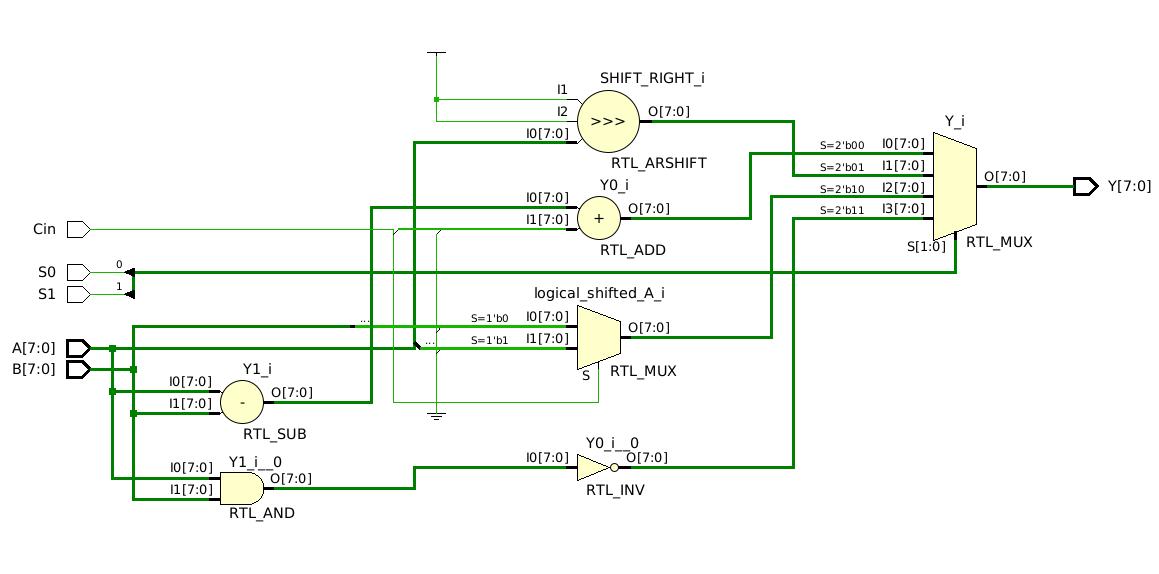
\includegraphics[width=\textwidth]{./images/alu-1/RLT_ALU.png}
\end{center}

Τρέχοντας την προσομοίωση, προκύπτει η παρακάτω κυματομορφή:
\begin{center}
	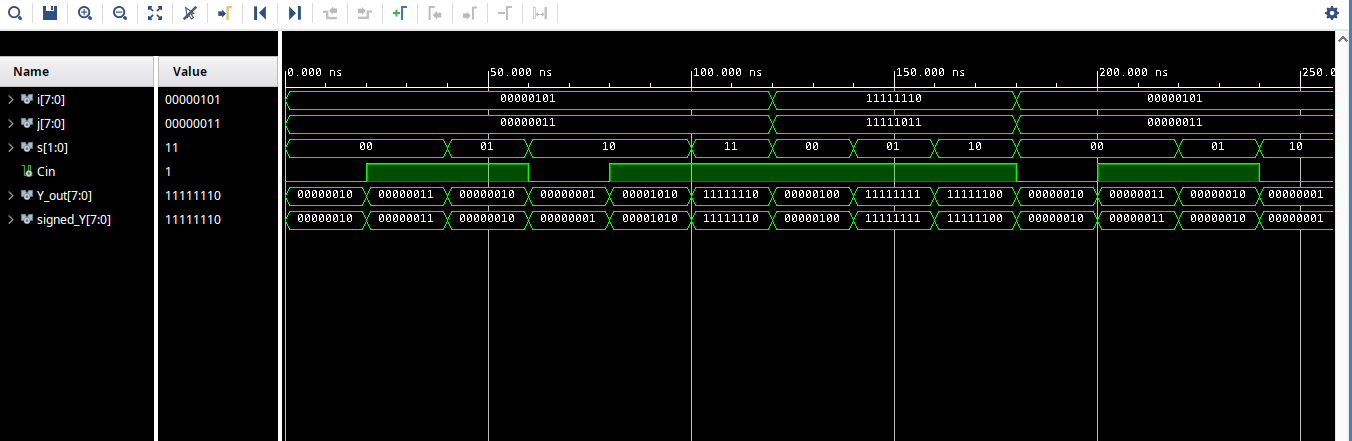
\includegraphics[width=\textwidth]{./images/alu-1/Behavioral_Sim_Fixed.png}
\end{center}

Στην συνέχεια μπορούμε να κάνουμε σύνθεση, η οποία δημιουργεί το παρακάτω schematic:
\begin{center}
	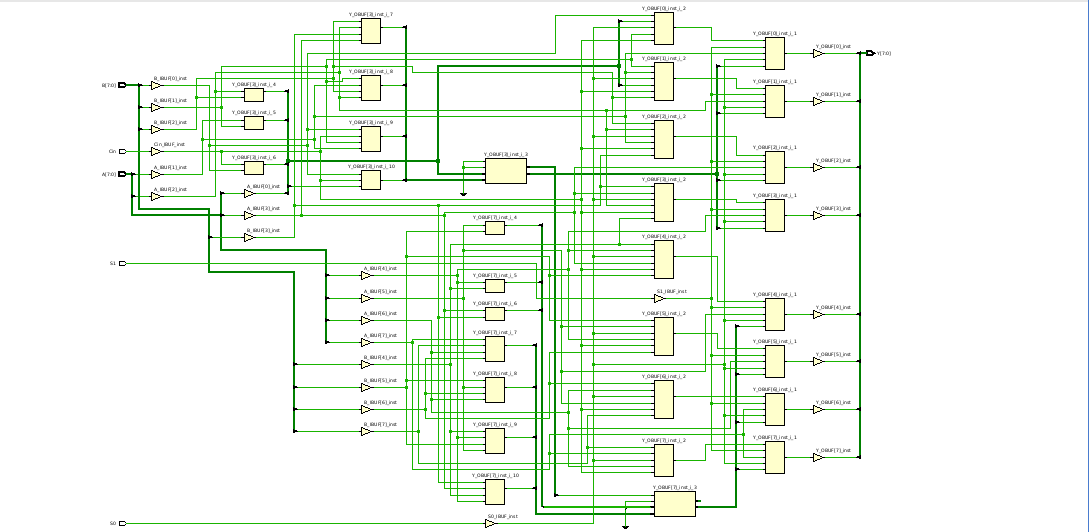
\includegraphics[width=\textwidth]{./images/alu-1/Synth_Schematic.png}
\end{center}

Μετά απο αυτό μπορεί να γίνει και Post-Synthesis Timing Simulation, η οποία δημιουργεί την παρακάτω κυματομορφή:
\begin{center}
	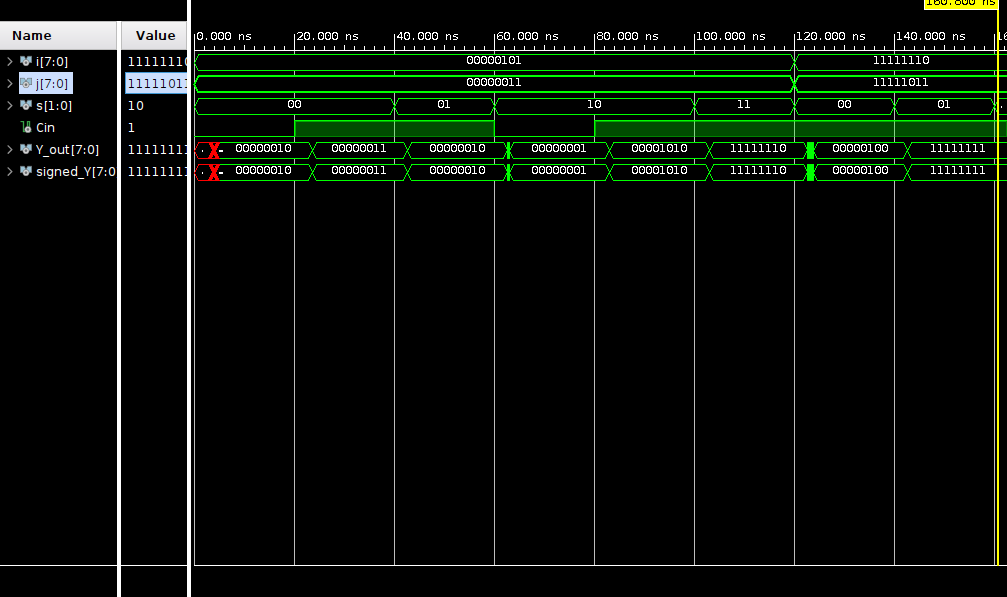
\includegraphics[width=\textwidth]{./images/alu-1/PST_Fixed.png}
\end{center}

Παρατηρούμε την σημαντική διαφορά ανάμεσα στην προσωμοίωση και το Post Synthesis Timing Simulation, ότι δηλαδή τα σήματα στο behavioural simulation αλλάζουν άμεσα, ενώ στο PSTS υπάρχει μια καθυστέρηση καθώς και θόρυβος κατά την μεταβολή του σήματος.

Μπορούμε να βρούμε τους πόρους που χρησιμοποιεί η υλοποίησή μας, χρησιμοποιούμε το Report Utilization το οποίο παράγει τον παρακάτω πίνακα:
\begin{center}
	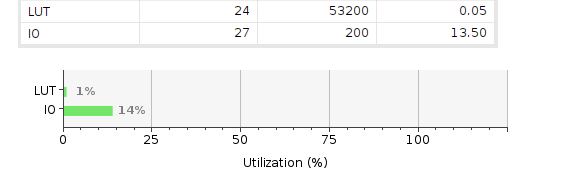
\includegraphics[width=\textwidth]{./images/alu-1/Utilization.png}
\end{center}

Αυτό σημαίνει ότι χρησιμοποιούμε 24 lookup tables και 27 IO buffers για ενίσχυση του εισερχόμενου ή εξερχόμενου σήματος.

Τέλος, μπορούμε να κάνουμε Report Timings και πηγαίνοντας στο Summary να δούμε τα παρακάτω σχετικά με τις καθυστερήσεις διάδοσης και μόλυνσης αντίστοιχα:
\begin{center}
	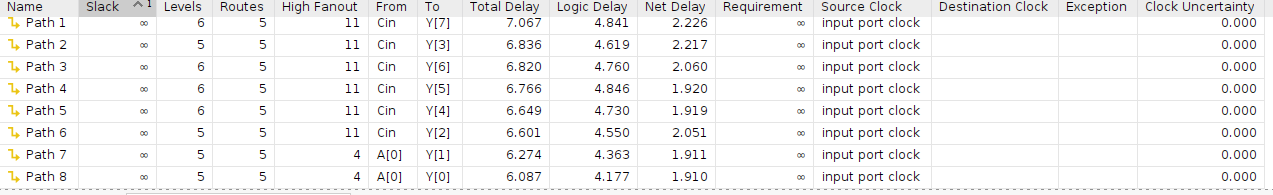
\includegraphics[width=\textwidth]{./images/alu-1/Setup_Time_Summury.png}
	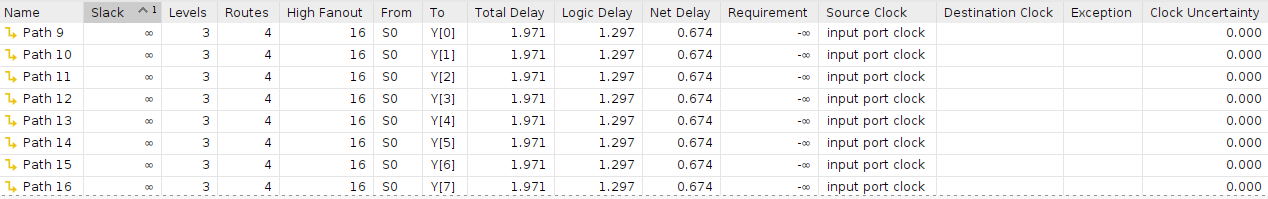
\includegraphics[width=\textwidth]{./images/alu-1/Hold_Time_Summury.png}
\end{center}

Από το παραπάνω, κάνοντας διπλό κλικ στο πιο αργό και στο πιο γρήγορο μονοπάτι αντίστοιχα, μπορούμε να τα δούμε πάνω στο σχεδιάγραμα:
\begin{center}
	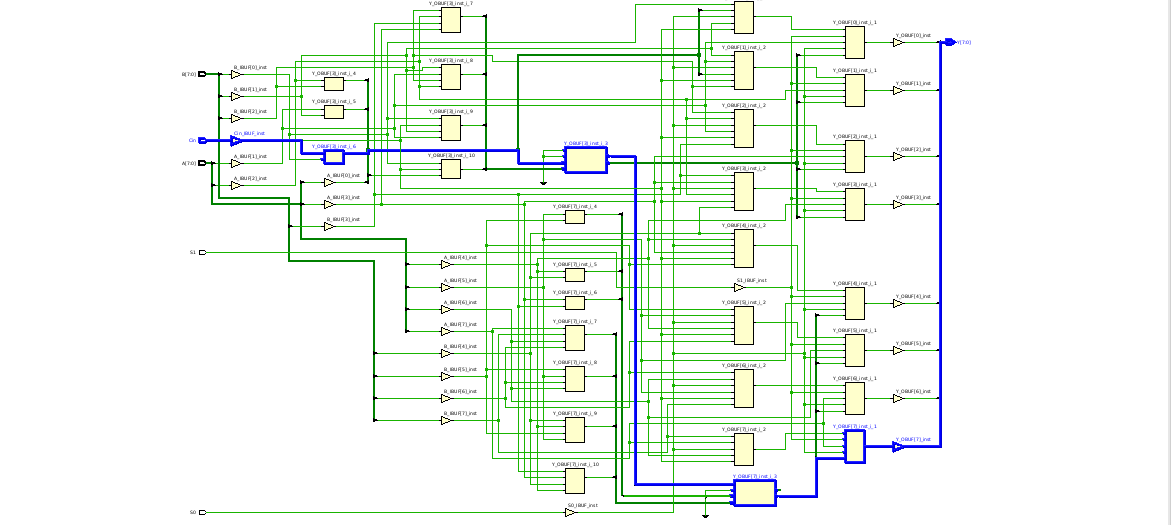
\includegraphics[width=\textwidth]{./images/alu-1/Slowest_Path.png}
	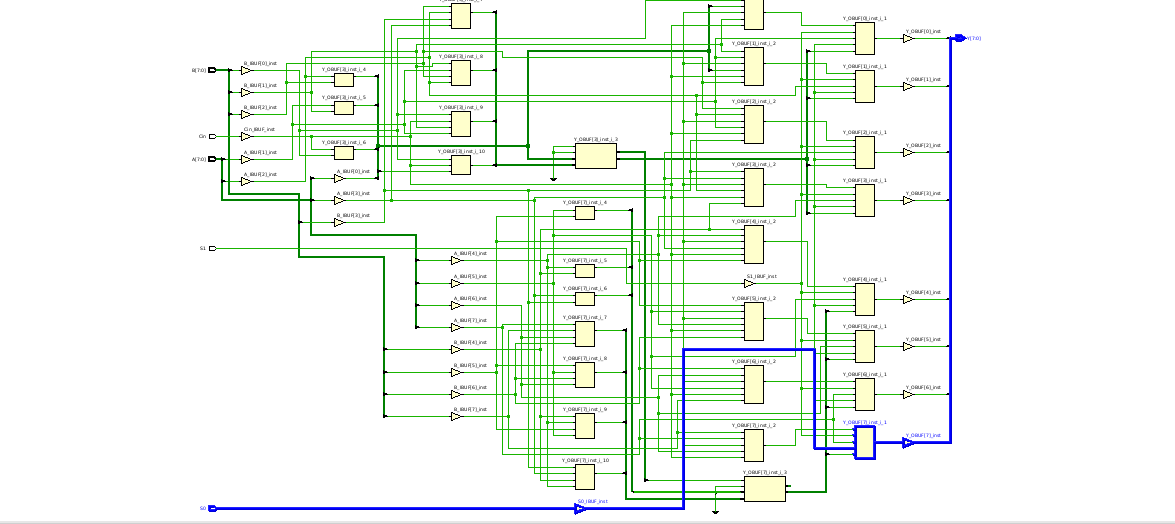
\includegraphics[width=\textwidth]{./images/alu-1/Fastest_Path.png}
\end{center}


Το πιο αργό μονοπάτι παρατηρούμε ότι είναι αυτό που ξεκινά από το $C_{in}$ σήμα και πήγαινει στην έξοδο, περνώντας από μονάδες τύπου CarryLogic.
Αντίστοιχα, το πιο γρήγορο μονοπάτι είναι από το δεύτερο bit του σήματος ελέγχου μέχρι την έξοδο, πράγμα λογικό μιας που το $S_0$ χρησιμοποιείται μόνο ως σήμα ελέγχου πολυπλέκτη και δεν συμμετέχει σε λογική.

\section{Άσκηση 2}
Για την υλοποίηση της περιγραφόμενης ALU θα ξεκινήσουμε οργανώνοντας τις περιπτώσειςε εκτέλεσης.
Αν $C_{1:0}$ είναι το σήμα ελέγχου της ALU, τότε:
\begin{center}
  \begin{tabular}{|c|c|c|}
    \hline
    $C_1$ & $C_0$ & Πράξη \\
    \hline
    0 & 0 & rol \\
    0 & 1 & ror \\
    1 & 0 & srl \\
    1 & 0 & sll \\
    \hline
  \end{tabular}
\end{center}

Μπορούμε να ομαδοποιήσουμε τις παραπάνω περιπτώσεις, παρατηρώντας ότι το πρώτο bit $C_1$ του Control σήματος, ελέγχει το είδος της πράξης που θα εκτελεστεί.
Αν είναι $0$ τότε εκτελείται περιστροφή(rotation), διαφορετικά εκτελείται ολίσθηση(shift).
Αντίστοιχα το δεύτερο bit ελέγχει την κατεύθυνση της περιστροφής ή της ολίσθησης. Ωστόσο, η επίδραση του διαφέρει από την μία περίπτωση στην άλλη.
Το δεύτερο bit δηλαδή αν γίνεται περιστροφή, είναι $1$ όταν η περιστροφή είναι δεξιόστροφη και $0$ όταν είναι αριστερόστροφη.
Αντίθετα, όταν γίνεται ολίσθηση, είναι $1$ όταν πρόκειται για αριστερή ολίσθηση και $0$ όταν πρόκειται για δεξιά.
Συνεπώς μπορούμε να περιγράψουμε το αποτέλεσμα της μονάδας ως εξής:
\begin{itemize}
  \item Αν $C_1 = 0$, τότε:
    \begin{itemize}
      \item Αν $C_0 = 0$ κάνε αριστερή περιστροφή.
      \item διαφορετικά κάνε δεξιά περιστροφή
    \end{itemize}
  \item διαφορετικά,
    \begin{itemize}
      \item Αν $C_0 = 0$ κάνε δεξιά ολίσθηση,
      \item διαφορετικά κάνε αριστερή περιστροφή.
    \end{itemize}
\end{itemize}

Το παραπάνω παραπέμπει στην χρήση ενός πολυπλέκτη 4-σε-1.

\subsection{Dataflow}
Στην Dataflow αρχιτεκτονική, δεν μπορούμε να χρησιμοποιήοσυμε εξωτερικές οντότητες και processes.
Αρχικά θα δημιουργήσουμε δύο εσωτερικά σήματα που θα περιέχουν τα αποτελέσματα των δύο πράξεων.
Για να δώσουμε τιμή στα σήματα, θα χρησιμοποιήσουμε ανάθεση υπό συνθήκη, χρησιμοποιώντας ως συνθήκη το δεύτερο bit του σήματος Control($C_1$).
Στην συνέχεια, αρκεί να δώσουμε στην έξοδο $Result$ ως αποτέλεσμα το αποτέλεσμα της επιλεχθήσας πράξης, πράγμα που υλοποιείται επίσης με ανάθεση υπο συνθήκη, αυτή την φορά με συνθήκη το πρώτο bit του σήματος ελέγχου($C_0$).

Το παραπάνω έχει ως αποτέλεσμα, μια αρχιτεκτονική με τον παρακάτω κώδικα:
\inputminted[breaklines, linenos, firstline=12, lastline=30]{vhdl}{./code/part-2/alu-2/alu.vhdl}

Παρατηρούμε την διαφοροποίηση μεταξύ των τιμώς των σημάτων \mintinline{vhdl}{shifted_a} και \mintinline{vhdl}{rotated_a} είναι ο τρόπος που γεμίζονται τα ελεύθερα bit που δημιουργούνται μετά από ολίσθηση, καθώς και ο τρόπος που το δεύτερο bit επηρεάζει το αποτέλεσμα.

\subsection{Behavioural}
Για την υλοποίηση μιας αντίστοιχης behavioural αρχιτεκτονικής, μπορούμε να χρησιμοποιήσουμε processes.
Χρησιμοποιούμε 3 processes(μπορούσαμε και 1):
\begin{enumerate}
  \item \mintinline{vhdl}{shift}: Αυτό το process εφαρμόζει τους κανόνες της ολίσθησης και δίνει στο εσωτερικό σήμα \mintinline{vhdl}{shifted_a} τιμή το αποτέλεσμα της ολίσθησης του $a$.
  \item \mintinline{vhdl}{rotate}: Αυτό το process εφαρμόζει τους κανόνες της περιστροφής και δίνει στο εσωτερικό σήμα \mintinline{vhdl}{rotated_a} τιμή το αποτέλεσμα της ολίσθησης του $a$.
  \item Ένα τελικό process, που δίνει στο $Result$ σήμα, τιμή ανάλογα με την τιμή του πρώτου bit του σήματος ελέγχου.
\end{enumerate}

Σημαντική παρατήρηση είναι ότι η λίστα ευαισθησίας των processes \mintinline{vhdl}{shift} και \mintinline{vhdl}{rotate}, υπάρχει το $a$ και το δεύτερο bit του σήματος ελέγχου(αφού επηρεάζει το αποτέλεσμά τους), ενώ στο τελευταίο process, το πρώτο bit του σήματος ελέγχου καθώς και τα σήματα \mintinline{vhdl}{shifted_a} και \mintinline{vhdl}{rotated_a} δηλαδή οι έξοδοι των άλλων processes.
Ο κώδικας που προκύπτει είναι ο παρακάτω:
\inputminted[breaklines, linenos, firstline=32, lastline=62]{vhdl}{./code/part-2/alu-2/alu.vhdl}

\subsection{Structural}
Η structural αρχιτεκτονική πρέπει να χρησιμοποιεί δύο ακόμη οντότητες. Έναν περιστροφέα κι έναν ολισθητή.
Η υλοποίησή τους είναι σχετικά εύκολη και μπορεί να γίνει με αντιγραφή του κώδικα που δίνει τιμές στα σήματα \mintinline{vhdl}{shifted_a} και \mintinline{vhdl}{rotated_a} από την dataflow αρχιτεκτονική.
\inputminted[breaklines, linenos]{vhdl}{./code/part-2/alu-2/shiftlr_4bit.vhdl}
\inputminted[breaklines, linenos]{vhdl}{./code/part-2/alu-2/rotatelr_4bit.vhdl}

Στην συνέχεια, αρκεί να δηλώσουμε components για τις οντότητες αυτές και να συνδέσουμε κατάλληλα τα εσωτερικά σήματα.
Αποτέλεσμα των παραπάνω είναι ο παρακάτω κώδικας:
\inputminted[breaklines, linenos, firstline=64]{vhdl}{./code/part-2/alu-2/alu.vhdl}

\newpage

\begin{figure}
  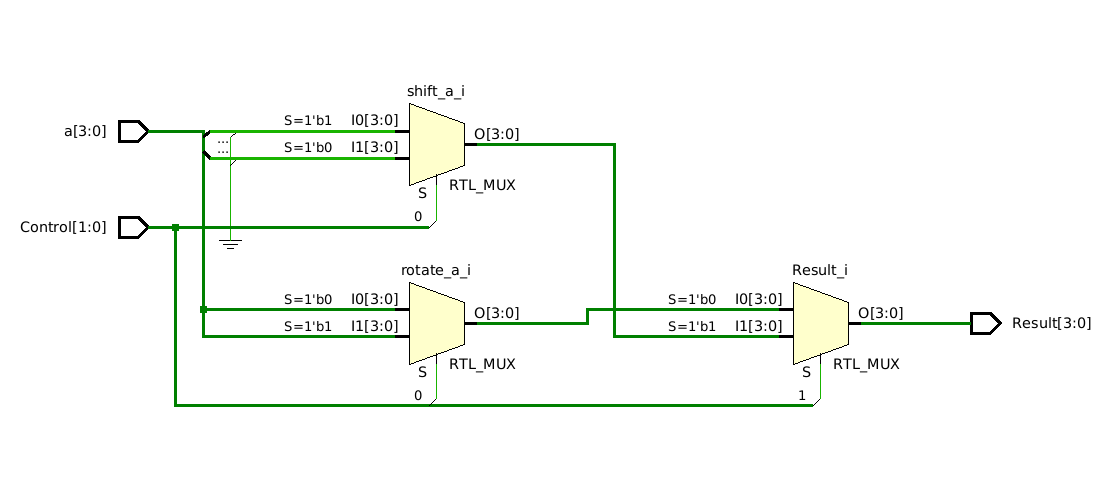
\includegraphics[width=\textwidth]{./images/alu-2/RLT_DF_2.png}
  \caption{RTL διάγραμμα της Dataflow αρχιτεκτονικής}
  \label{fig:df}
\end{figure}

\begin{figure}
  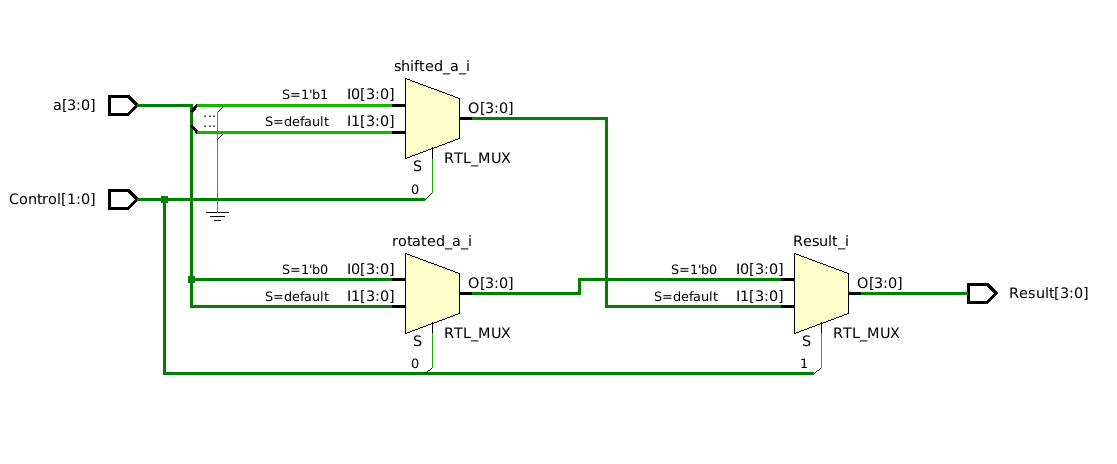
\includegraphics[width=\textwidth]{./images/alu-2/RTL_Beh_2.png}
  \caption{RTL διάγραμμα της Behavioural αρχιτεκτονικής}
  \label{fig:beh}
\end{figure}

\begin{figure}
  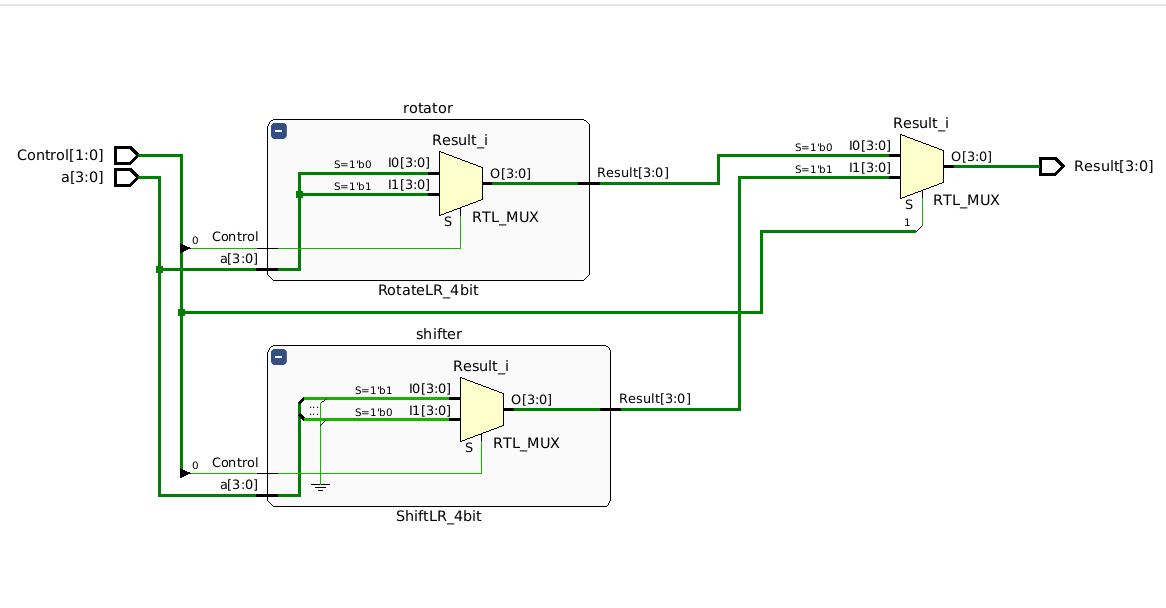
\includegraphics[width=\textwidth]{./images/alu-2/RTL_ALU_2.png}
  \caption{RTL διάγραμμα της Structural αρχιτεκτονικής}
  \label{fig:struct}
\end{figure}

\begin{figure}
  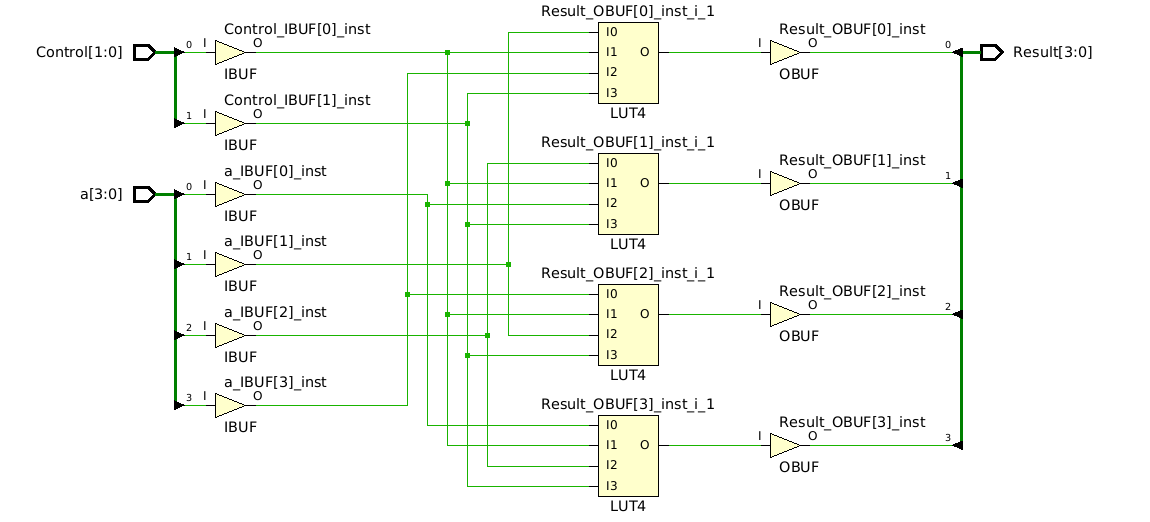
\includegraphics[width=\textwidth]{./images/alu-2/Synth_Schem_ALU_2.png}
  \caption{Διάγραμμα που προκύπτει μετά την φάση της σύνθεσης. Και οι τρεις αρχιτεκτονικές υλοποιούν την ίδια λογική και για αυτό το διάγραμμα της σύνθεσης είναι ίδιο για όλες τους}
  \label{fig:synth}
\end{figure}

Μπορούμε τώρα να προχωρίσουμε στην φάση της RTL ανάλυσης. Στα σχήματα \ref{fig:df}, \ref{fig:beh}, \ref{fig:struct} φαίνονται τα διαγράμματα που προκύπτουν.
Κατά την φάση της σύνθεσης, το schematic που προκύπτει είναι ίδιο για όλες τις αρχιτεκτονικές και φαίνεται στο σχήμα \ref{fig:synth}

Μπορούμε και να κάνουμε προσομοίωση. Το αρχείο της προσομοίωσης μπορεί να ελέγξει και τις τρεις αρχιτεκτονικές ταυτόχρονα.
Η κυματομορφή που προκύπτει από την προσομοίωση για τιμή Control = 0, φαίνεται στο σχήμα \ref{fig:beh_wfm_0}. 
Η κυματομορφή που προκύπτει από την εκτέλεση μόνος της αρχιτεκτονικής Dataflow, φαίνεται στο σχήμα \ref{fig:beh_overview} για όλες τις τιμές του Control σήματος.
Το αρχείο \mintinline{vhdl}{alu_tb_simple.vhdl} μπορεί να χρησιμοποιηθεί για την δημιουργία αντίστοιχων κυματομορφών για τις άλλες αρχιτεκτοτινκές.

\begin{figure}
  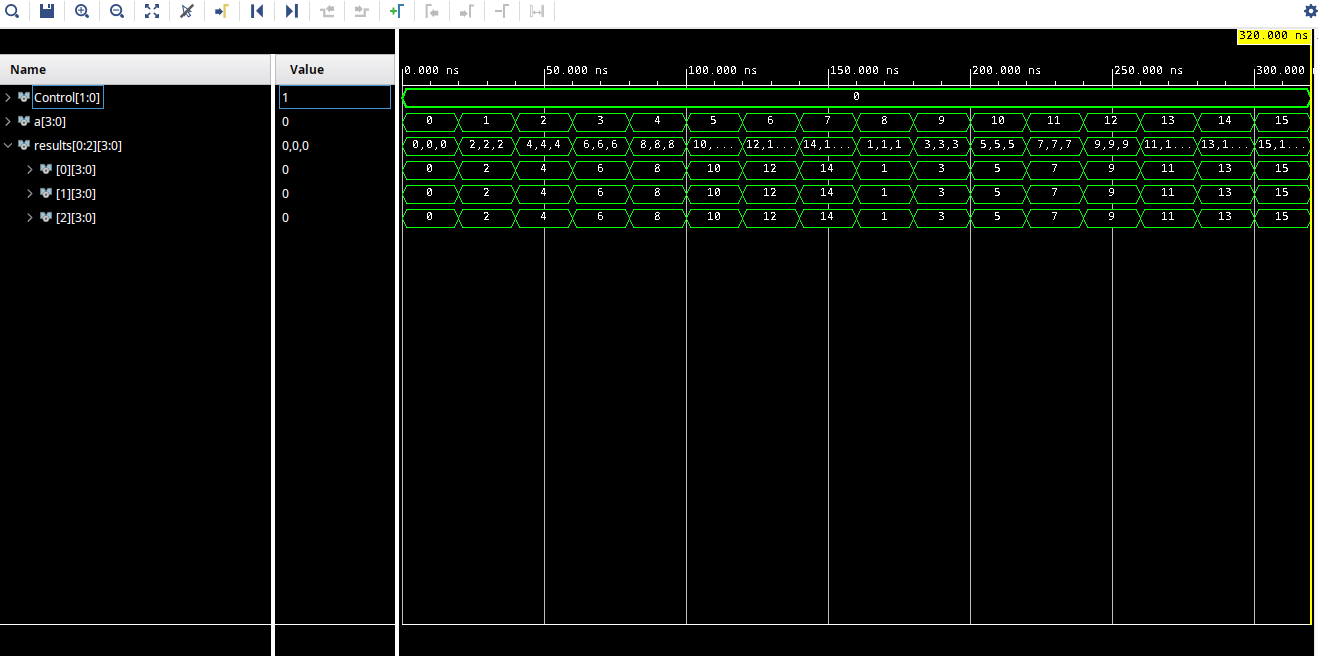
\includegraphics[width=\textwidth]{./images/alu-2/beh-sim-0.png}
  \caption{Waveform από Behavioural Simulation για Control = 0. Το results(0) είναι το αποτέλεσμα της dataflow αρχιτεκτονικής, το results(1) της behavioural και το results(2) της structural}
  \label{fig:beh_wfm_0}
\end{figure}

\begin{figure}
  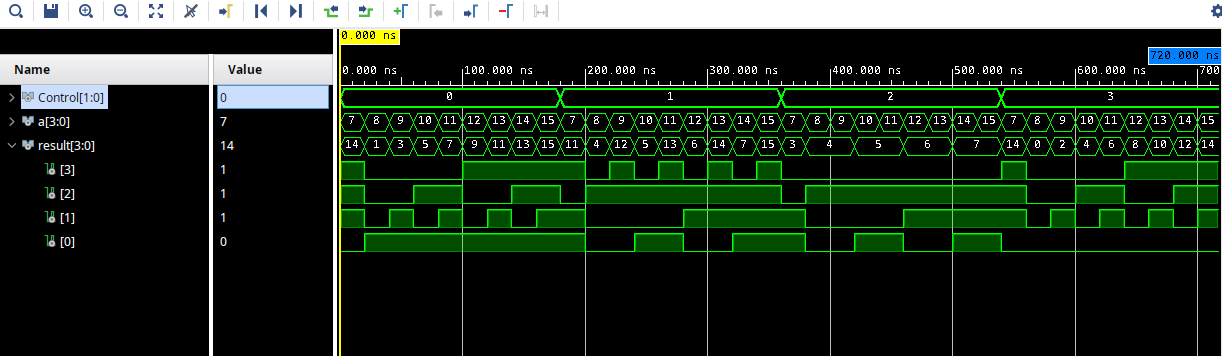
\includegraphics[width=\textwidth]{./images/alu-2/beh-sim-overview.png}
  \caption{Waveform από behavioural simulation με την χρήση του alu\_tb\_simple αρχείου προσομοίωσης}
  \label{fig:beh_overview}
\end{figure}

\newpage

\begin{figure}
  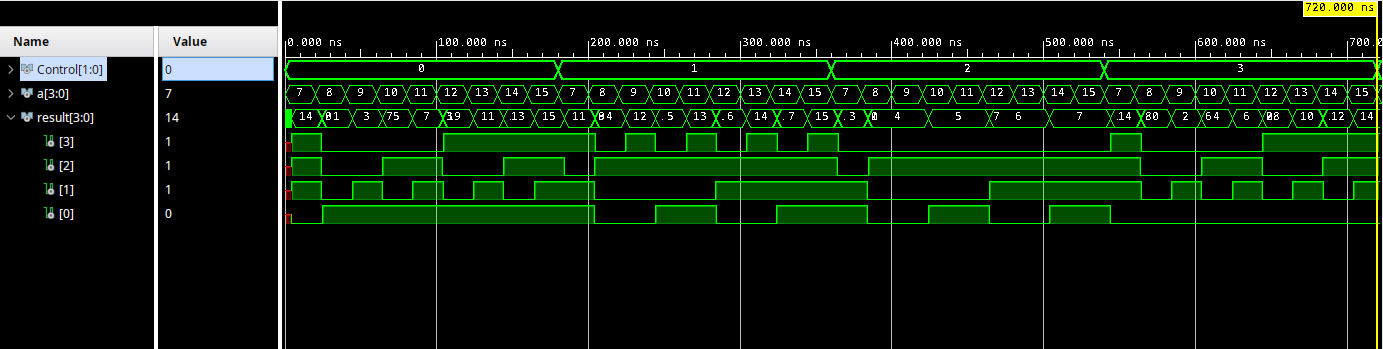
\includegraphics[width=\textwidth]{./images/alu-2/pits.png}
  \caption{Waveform που προκύπτει από το Post implementation timing simulation με την χρήση του alu\_tb\_simple αρχείου προσομοίωσης}
  \label{fig:pits}
\end{figure}

\begin{figure}
  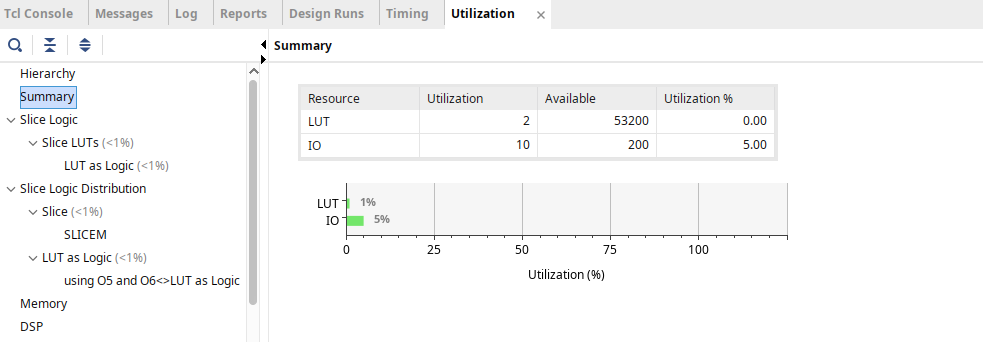
\includegraphics[width=\textwidth]{./images/alu-2/impl-util.png}
  \caption{Utilization report μετά από implementation}
  \label{fig:util}
\end{figure}

Μπορούμε τώρα να περάσουμε στο στάδιο του implementation. Με την χρήση του \mintinline{vhdl}{alu_tb_simple.vhdl} μπορούμε για όποια αρχιτεκτονική θέλουμε να τρέξουμε Post implementation timing simulation.
Η κυματομορφή που προκύπτει είναι ίδια για όλες τις αρχιτεκτονικές, αφού το schematic που προκύπτει είναι ίδιο και φαίνεται στο σχήμα \ref{fig:pits}. 
Παρατηρούμε 3 σημαντικές διαφορές ανάμεσα στο σχήμα \ref{fig:pits} και στο σχήμα \ref{fig:beh_overview}:
\begin{enumerate}
  \item Στο Post-Implementation timing simulation, το σήμα result ξεκινά έχοντας την τιμή 'X' και μετά από ένα μικρό χρονικό διάστημα, παίρνει δεκτή μορφή, ενώ στο behavioural simulation, ξεκινά από την αρχή με την τιμή 7 την οποία ελέγχει πρώτη η προσομοίωση.
  \item Στο Post-Implementation timing simulation, κατά την αλλαγή των τιμών εισόδου, δεν γίνεται ακαριαία η αλλαγή στις τιμές εξόδου και υπάρχει καθυστέρηση, η οποία δεν εμφανίζεται στο behavioural simulation.
  \item Στο Post-Implementation timing simulation, η τιμή της εξόδου δεν παίρνει αμέσως την τελική της τιμή αλλά επηρεάζεται από θόρυβο, πράγμα που επίσης δεν συμβαίνει στο behavioural simulation.
\end{enumerate}

Κάνοντας report utilization  προκύπτει το σχήμα \ref{fig:util} από το οποίο φαίνεται ότι χρησιμοποιούμε 2 lookup tables των 10 IO buffers.
Τέλος, κάνοντας timing report, μπορούμε να βρούμε τις καθυστερήσεις διάδοσης και μόλυνσης κάνοντας report timings.
Από αυτό προκύπτει οι πίνακες που φαίνονται στα σχήματα \ref{fig:slow} και \ref{fig:fast} και αντίστοιχα η αργότερη διαδρομή(σχήμα \ref{fig:slow_path}) και η γρηγορότερη(σχήμα \ref{fig:fast_path}) διαδρομή του κυκλώματος.
Παρατηρούμε, ότι παρόλο που όλα τα σήματα περνούν από τον ίδιο αριθμό επιπέδων λογικής, τα σήματα Control έχουν πιο γρήγορες διαδρομές από τα σήματα εισόδου.
Αυτό πιθανό να οφείλεται στον τρόπο που υλοποιούνται τα lookup tables, μιας που στην πραγματικότητα πρόκειται για πολυπλέκτες. Αφού το σήμα Control χρησιμοποιείται ως σήμα ελέγχου, πιθανό να υπάρχει κάποιος αποδοτικός τρόπος για την υλοποίηση του στο υλικό, ο οποίος είναι πιο γρήγορος από την χρήση πίνακα αληθείας(που γίνεται συνήθως κατά την υλοποίηση συνδυαστικής λογικής σε lookup tables).

\begin{figure}
  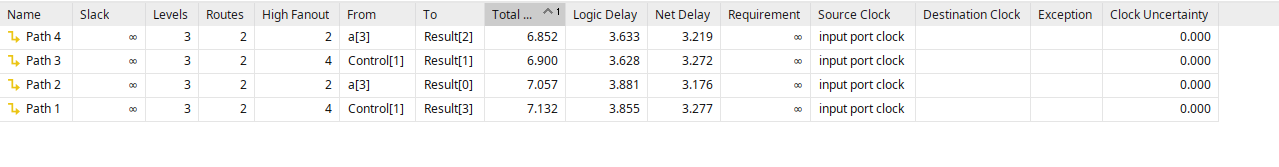
\includegraphics[width=\textwidth]{./images/alu-2/slow-report.png}
  \caption{Setup times από τα οποία φαίνεται ότι η καθυστέρηση διάδοσης του κυκλώματος είναι 6.852 ns}
  \label{fig:slow}
\end{figure}

\begin{figure}
  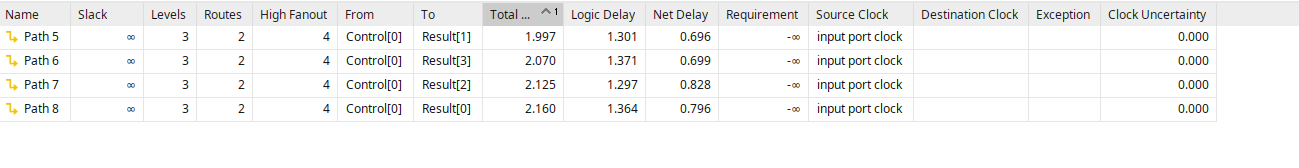
\includegraphics[width=\textwidth]{./images/alu-2/fast-report.png}
  \caption{Hold times από τα οποία φαίνεται ότι η καθυστέρηση μόλυνσης του κυκλώματος είναι 1.997 ns}
  \label{fig:fast}
\end{figure}

\begin{figure}
  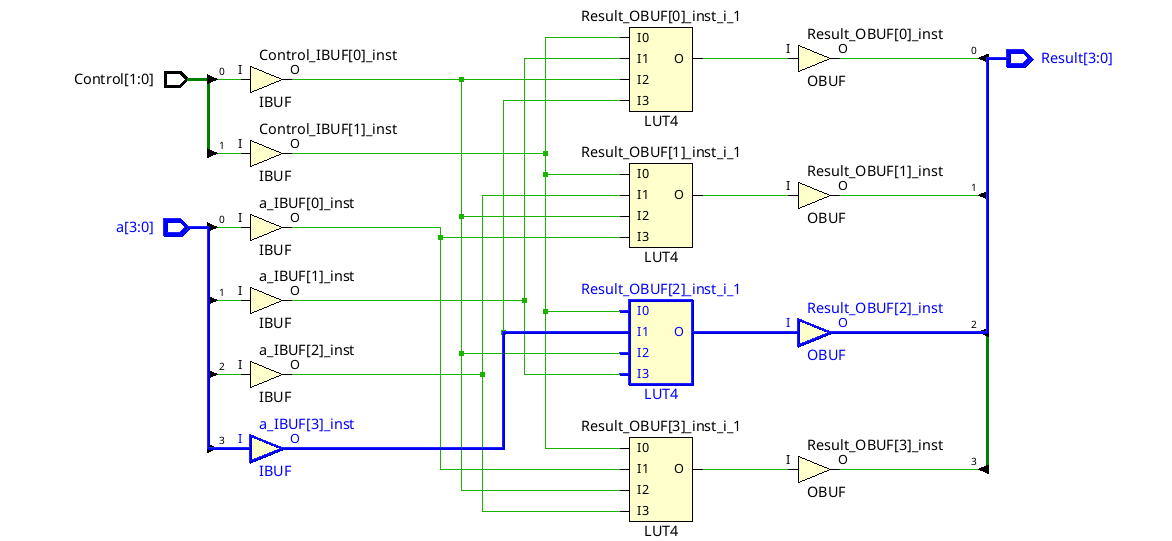
\includegraphics[width=\textwidth]{./images/alu-2/slow-path.png}
  \caption{Αργότερη διαδρομή του κυκλώματος που καθορίζει την καθυστέρηση διάδοσης}
  \label{fig:slow_path}
\end{figure}

\begin{figure}
  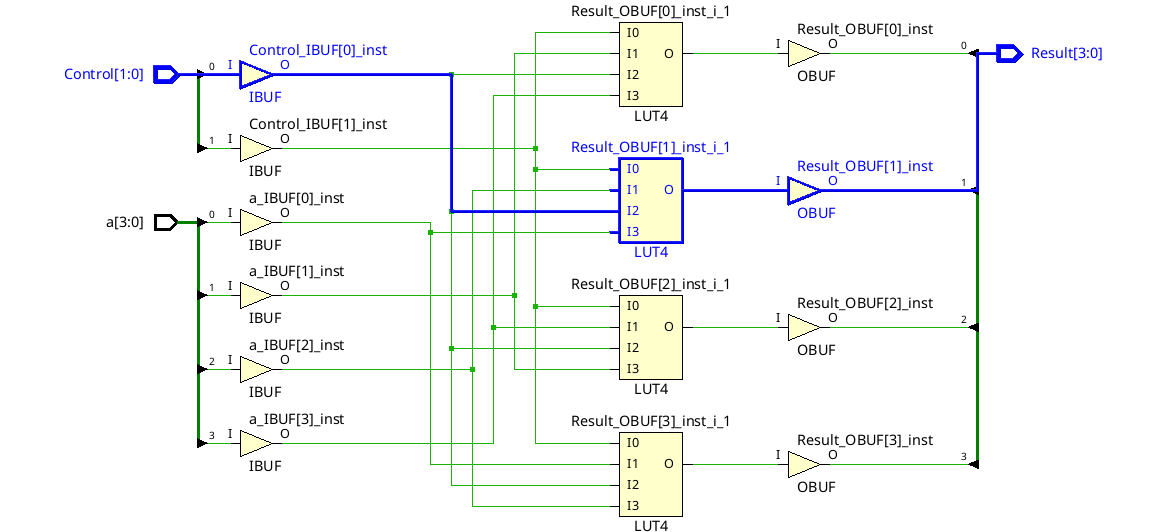
\includegraphics[width=\textwidth]{./images/alu-2/fast-path.png}
  \caption{Γρηφορότερη διαδρομή του κυκλώματος που καθορίζει την καθυστέρηση μόλυνσης}
  \label{fig:fast_path}
\end{figure}

\end{document}
